\documentclass[a4paper,12pt]{article}

\usepackage[spanish]{babel}
\usepackage{listings}
\usepackage[utf8]{inputenc}
\usepackage{titling}
\usepackage{enumitem}
\usepackage{fancyhdr}
\usepackage{xcolor}
\usepackage{geometry}
\usepackage{graphicx}
\usepackage{hyperref}
\usepackage{cite}
\usepackage{url}
\usepackage{fix-cm}
\usepackage{tikz}
\usepackage{etoolbox}
\usepackage[format=plain,
            labelfont={bf,it},
            textfont=it]{caption}
\usetikzlibrary{positioning}
\usetikzlibrary{arrows.meta}
\usetikzlibrary{calc}

\patchcmd{\thebibliography}{\section*{\refname}}{}{}{}

%%search -> (?:url=\{)(.*)(:?\})
%%replace -> howpublished={\\url{$1}}
%\geometry{a4paper, left=4em, right=4em, top=0em, bottom=4em}

\lstset{
    frame=single,
    breaklines=true,
    numbers=left,
    keywordstyle=\color{blue},
    numbersep=15pt,
    numberstyle=,
    basicstyle=\linespread{1.0}\selectfont\ttfamily,
    commentstyle=\color{gray},
    stringstyle=\color{orange},
    identifierstyle=\color{green!40!black},
}

\setlength{\parindent}{4em}
%%\setlength{\parindent}{0em}
\setlength{\parskip}{0.8em}
    
%%\renewcommand{\familydefault}{phv} %%Seleccionamos Helvetica
    
\lstdefinestyle{console}
{
    numbers=left,
    backgroundcolor=\color{violet},
    %%belowcaptionskip=1\baselineskip,
    breaklines=true,
    %%xleftmargin=\parindent,
    %%showstringspaces=false,
    basicstyle=\footnotesize\ttfamily,
    %%keywordstyle=\bfseries\color{green!40!black},
    %%commentstyle=\itshape\color{green},
    %%identifierstyle=\color{blue},
    %%stringstyle=\color{orange},
    basicstyle=\scriptsize\color{white}\ttfamily,
}

\newcommand{\size}[2]{{\fontsize{#1}{0}\selectfont#2}}
    
\title{Triángulo de Penrose}
%\subtitle{Diseño en 3D e implementación en OpenGL}
\date{}
\author{Aldán Creo Mariño}

\pagestyle{fancy}
\fancyhead[l]{Proyecto final}

\bibliographystyle{plain}
    
\begin{document}

\maketitle

\newpage
\tableofcontents
\newpage

\section{Concepto}
\subsection{El triángulo de Penrose}

El \textbf{triángulo de Penrose} es una figura imposible diseñada en 1934 por el artista sueco Oscar Reutersvärd. Sin embargo, no cobró notoriedad hasta 1954, cuando un matemático, Rodzher Penrouz (de ahí el nombre de la figura) escribió un artículo sobre figuras imposibles, que resultó muy llamativo. Desde ese momento pasó a formar parte de la cultura popular.

La figura tiene el aspecto mostrado en \ref{imagen_triangulo}.

\begin{figure}[h]
    \centering
    \resizebox*{0.4\textwidth}{!}{
    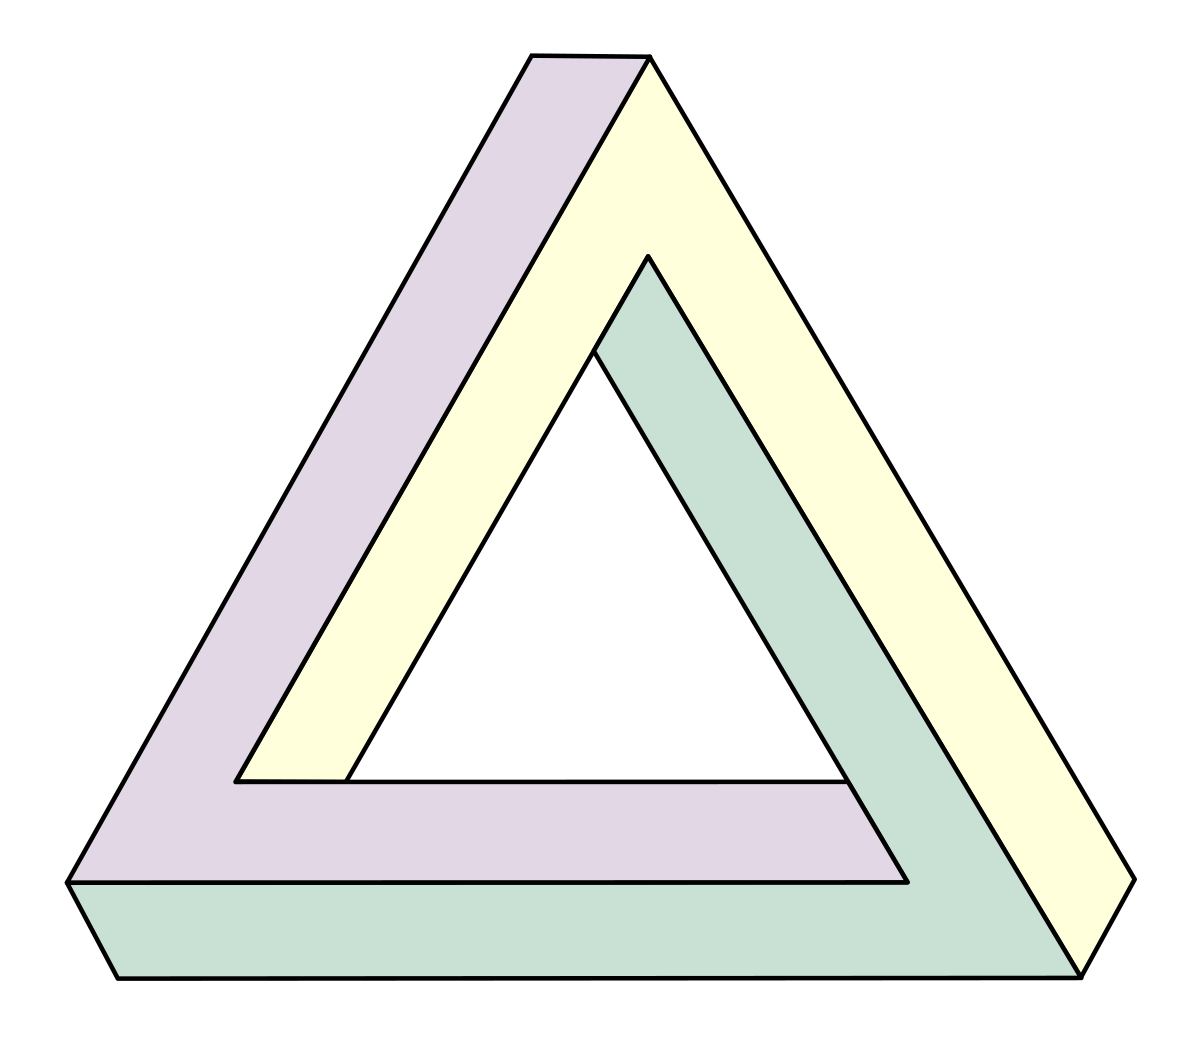
\includegraphics{1200px-Penrose_triangle.svg.png}
    }
    \caption{El triángulo de Penrose} \label{imagen_triangulo}
\end{figure}

A nivel personal, me resultan especialmente fascinantes todos los temas relacionados con figuras imposibles, y por eso quería que mi proyecto de la asignatura girase en torno a ellas. El triángulo de Penrose me pareció la figura más icónica que existe, entre las figuras imposibles, y por eso he desarrollado mi proyecto sobre la misma.

\subsection{Idea base para el desarrollo} \label{hocus}

Para hacer el desarrollo, me he basado en un juego de móvil llamado \textit{hocus} \cite{hocus}. El juego se basa en el uso de figuras imposibles, y concretamente tiene un nivel basado en el triángulo de Penrose, mostrado en \ref{nivel_hocus}.

\begin{figure}[h]
    \centering
    \resizebox*{0.4\textwidth}{!}{
    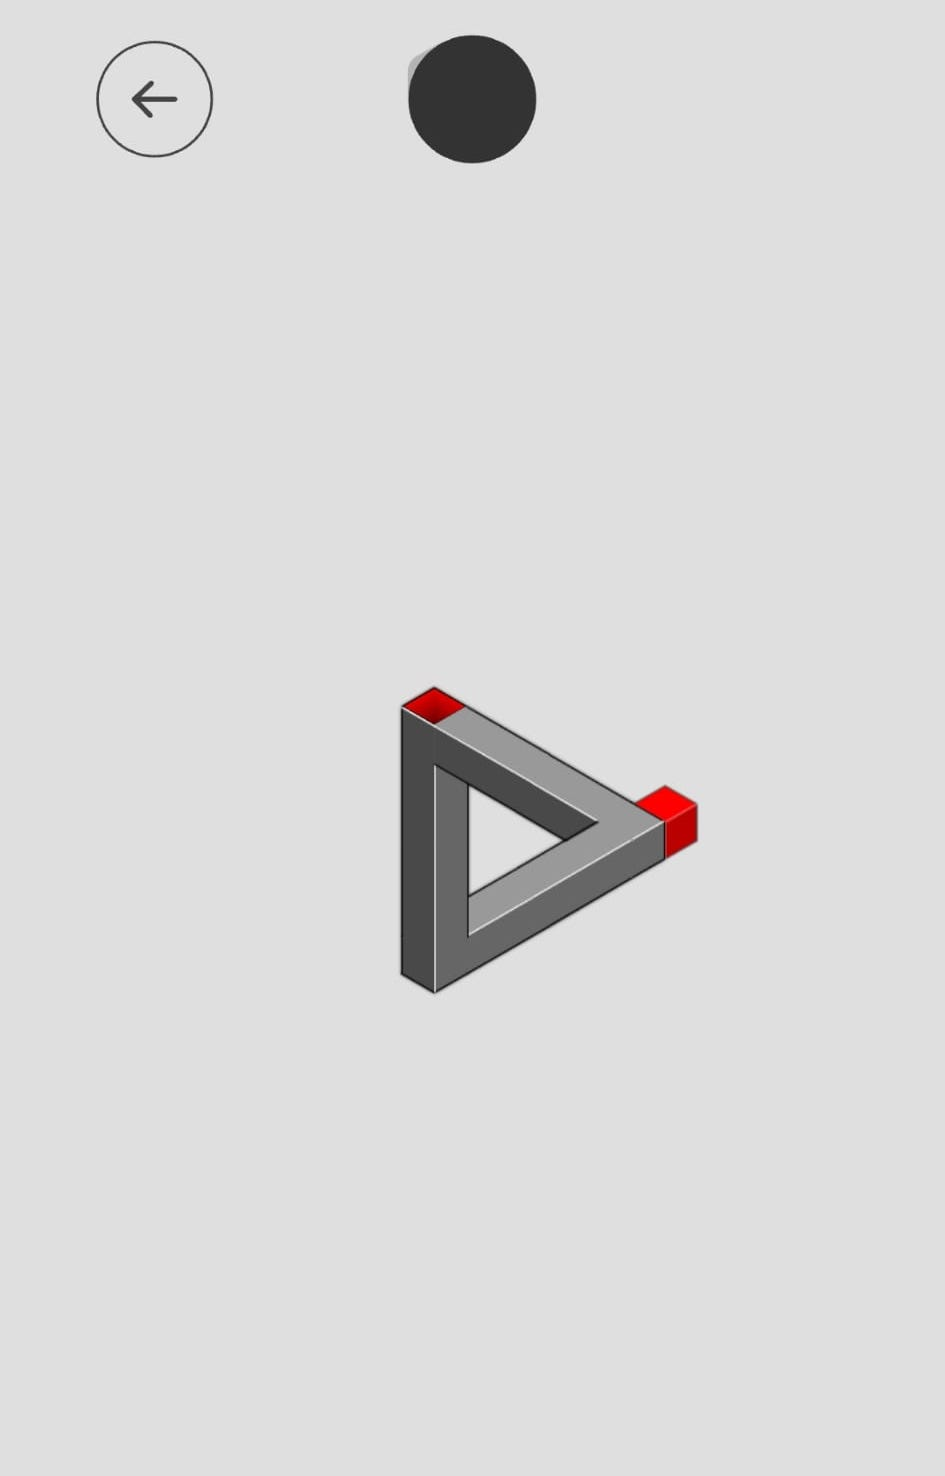
\includegraphics{hocus.jpeg}
    }
    \caption{Nivel 4 de \textit{hocus}} \label{nivel_hocus}
\end{figure}

Para diseñar la aplicación, he tratado de basar mi idea en la del diseño que han hecho en este juego, que sigue un estilo minimalista, y en el que se puede ver una figura que se va moviendo alrededor del triángulo de Penrose.

La idea que tomado para mi aplicación ha sido la misma: mostrar al usuario la ilusión óptica del triángulo de Penrose, con una esfera que va dando vueltas alrededor del mismo de una forma que es físicamente imposible.

\section{Diseño del modelo 3D}

\subsection{Obtención del modelo}

He comenzado con un modelo 3D disponible en \cite{modeloTriangulo}. Se trata de una página destinada a la impresión 3D, así que el modelo que ofrecían no era exactamente el apropiado para importar en la aplicación, ya que estaba adaptado para ser imprimible en el mundo real. Por eso tuve que editarlo de forma adecuada en Blender.

\subsection{Edición en Blender} \label{edicion_blender}

El modelo que descargué venía con todas las caras creadas, incluso las que en la aplicación aparecen ocultas. Esto, en principio, no debería suponer un problema, pero en la práctica sí lo es, cuando intento aplicar el algoritmo del pintor, que describiré en \ref{algoritmo_pintor}.

Por eso eliminé las caras ocultas del modelo, pasando de \ref{caras_ocultas_sin_borrar} a \ref{caras_ocultas_borradas}.

\begin{figure}[h]
    \centering
    \resizebox*{0.8\textwidth}{!}{
    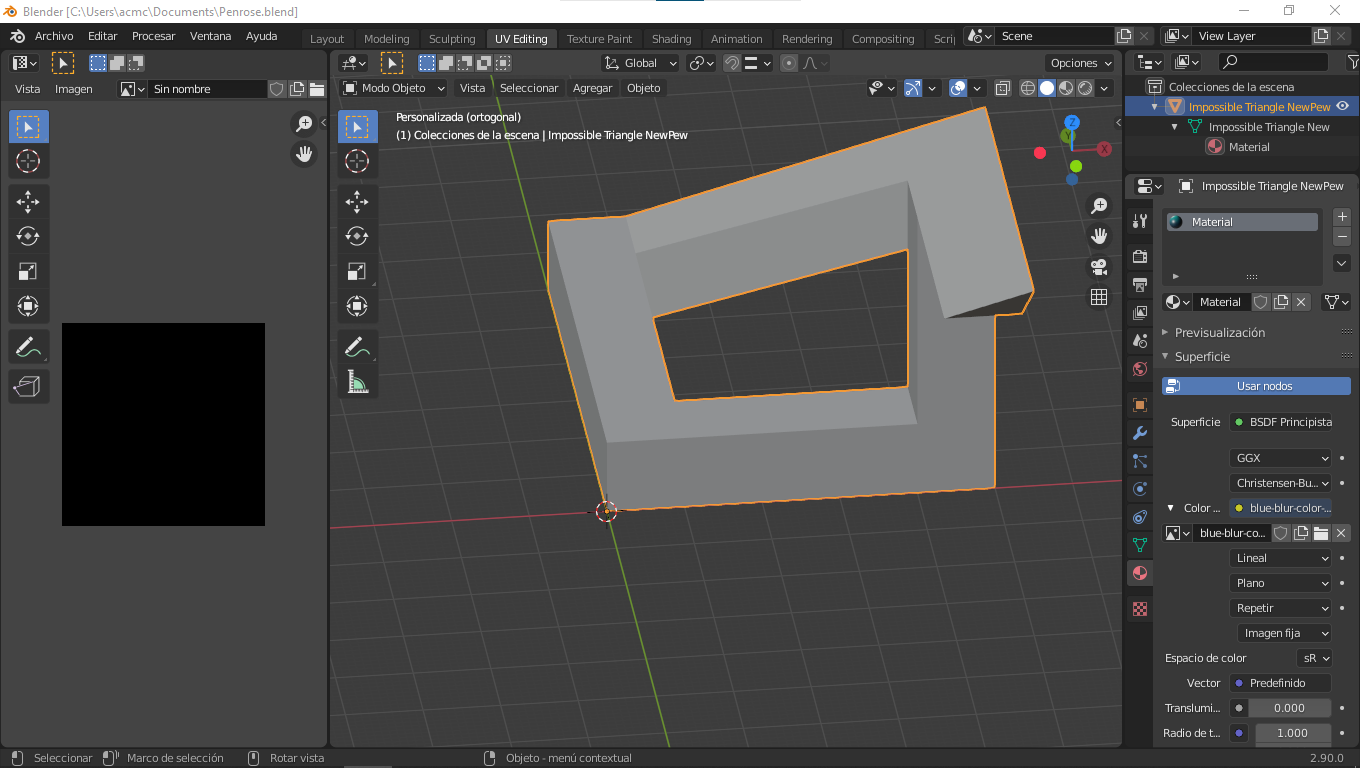
\includegraphics{caras_ocultas_sin_borrar.png}
    }
    \caption{Modelo original, con las caras ocultas sin borrar} \label{caras_ocultas_sin_borrar}
\end{figure}
\begin{figure}[h]
    \centering
    \resizebox*{0.8\textwidth}{!}{
    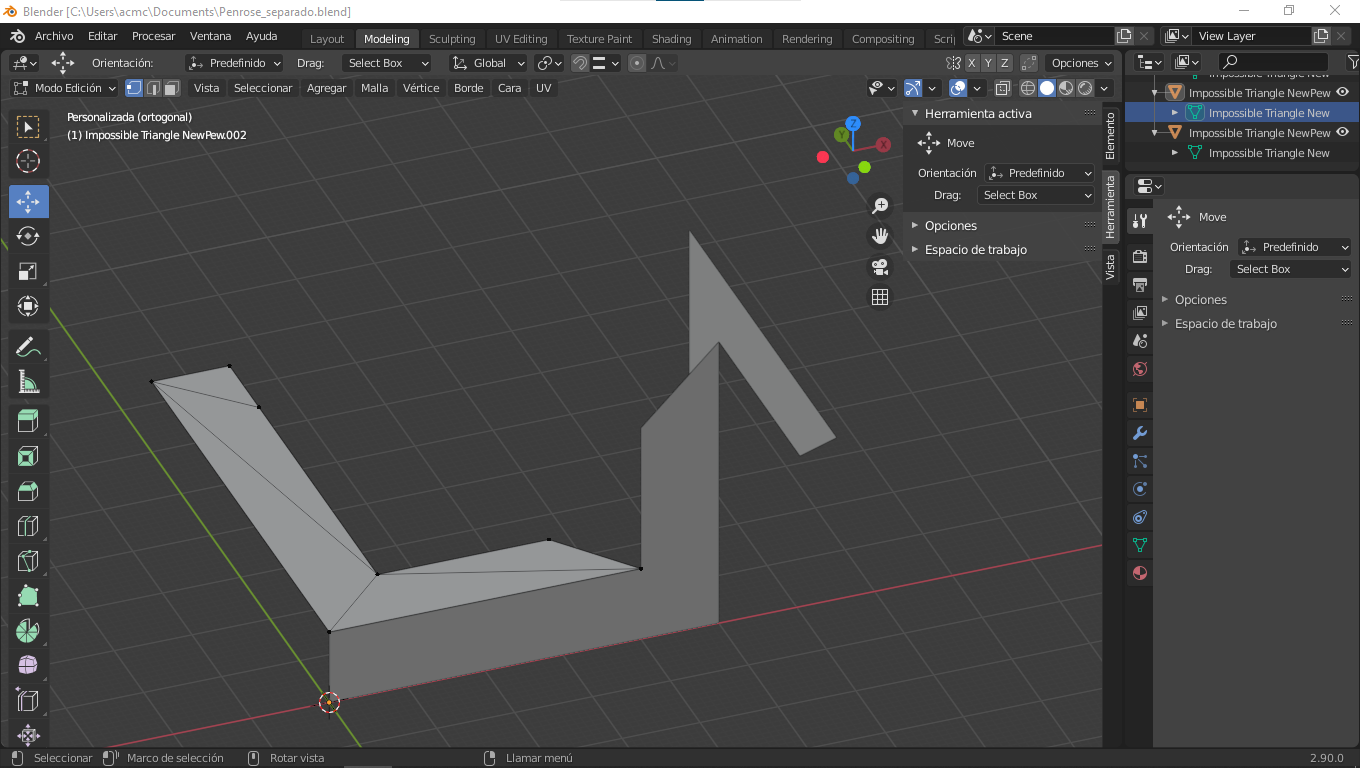
\includegraphics{caras_ocultas_borradas.png}
    }
    \caption{Modelo editado. Se han eliminado las caras ocultas y se ha separado en piezas.} \label{caras_ocultas_borradas}
\end{figure}

Además, separé las tres ``caras'' del triángulo, para poder aplicar después el algoritmo del pintor, según las secciones marcadas en rojo en \ref{separacion_caras_triangulo}, de forma aislada. Es relevante comentar que, en este documento, llamo ``caras'' a cada una de las tres mallas que he separado, por simplicidad. Técnicamente son mallas compuestas de múltiples caras.

\begin{figure}[h]
    \centering
    \resizebox*{0.6\textwidth}{!}{
    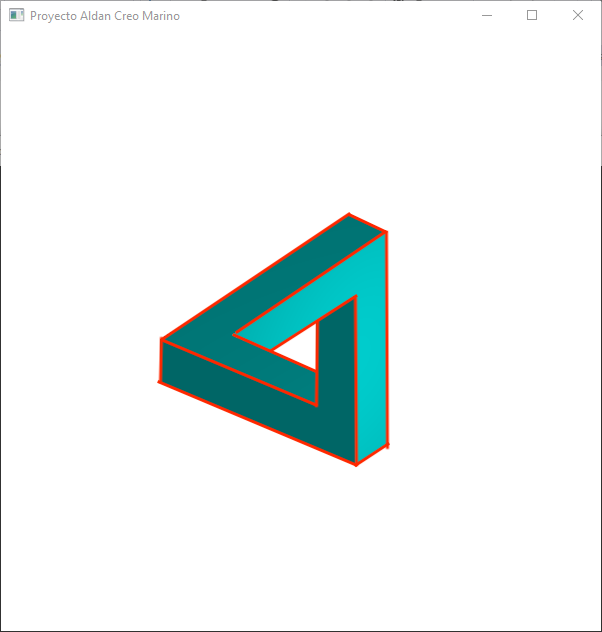
\includegraphics{caras_marcadas.png}
    }
    \caption{Separación de la malla en tres, vista desde la aplicación. Los límites de las caras están marcados en rojo.} \label{separacion_caras_triangulo}
\end{figure}

También hice el mapeado UV de las mallas, en caso de que quisiera aplicarle una textura posteriormente. Finalmente, deseché esa idea, ya que me pareció que quedaría recargado y sería más elegante un color más plano, como se ve en la versión final de la aplicación. La textura decidí aplicarla a la esfera (\ref{texturizado}).

\section{Programación de la aplicación con OpenGL}

En esta sección describiré como he llevado a cabo el proceso de programación de la aplicación, en el que he usado OpenGL 3.3.

\subsection{Estructura del código}

He estructurado mi código de forma similar a como he estructurado los códigos de las prácticas de la asignatura.

Concretamente, lo que hecho ha sido una estructura con un bucle de dibujo que se llama por cada frame que haya que dibujar, y que delega la responsabilidad de dibujar los objetos en clases que tienen precisamente ese propósito (es decir, tienen un método para realizar el dibujado de sí mismas). La información de cada objeto está encapsulada en la clase \texttt{Objeto}. Además, mantengo las funciones de crear los VAO, también de prácticas anteriores, y concretamente recurro al \texttt{esfera.h} que se nos proporcionó, para dibujar la esfera de la aplicación. La función de cargar una textura también es heredada de mi código de las prácticas.

Adicionalmente, he creado dos clases encargadas de controlar el movimiento de la esfera. Por un lado, tenemos una clase \texttt{Interpolador}, que describiré más adelante (\ref{interpolador}), y tenemos otra clase \texttt{ControladorEsfera}, que también describiré posteriormente (\ref{controlador_esfera}).

También heredo las funciones \texttt{openGLInit}, \texttt{window\_size\_callback}, etc.

\subsection{Importación del modelo del triángulo}

Desde Blender, exporté el modelo en formato \texttt{.obj}. Este formato permite leerlo de forma bastante directa desde OpenGL, pero tiene que ser procesado previamente. Mi primera intención sería intentar usar la librería de carga de modelos \texttt{Assimp}, que según leí en Internet es muy utilizada, pero como no estoy seguro de que esté permitido usar una librería externa en el proyecto, decidí procesar yo mismo el modelo para incorporarlo al código de la aplicación.

El formato del archivo es interpretable de forma bastante directa, así que utilicé expresiones regulares para convertir líneas de la forma \ref{lineas_obj} a vectores, como en \ref{lineas_obj_convertidas}.

\begin{figure}[h]
    \centering
    \begin{minipage}[c]{0.7\textwidth}
        \begin{lstlisting}
f 1/2/3 2/3/3 3/4/3
        \end{lstlisting}
    \end{minipage}
    \caption{Línea del fichero \texttt{.obj} que describe una cara.} \label{lineas_obj}
\end{figure}
\begin{figure}[h]
    \centering
    \begin{minipage}[c]{0.7\textwidth}
        \begin{lstlisting}
1, 2, 3, 2, 3, 3, 3, 4, 3,
        \end{lstlisting}
    \end{minipage}
    \caption{Línea convertida a formato vector de \texttt{unsigned int}s, para su uso directo en la aplicación. Corresponde a \ref{lineas_obj}.} \label{lineas_obj_convertidas}
\end{figure}

Utilicé el mismo procedimiento para todas las líneas, que son básicamente de cuatro tipos (vértices, caras, normales y texturizado).

De esta forma, construí un fichero \texttt{penrose.h}, basándome en el de las prácticas (\texttt{esfera.h}), con la información necesaria sobre la figura.

Pese a todo, como comentaba, realmente son tres mallas separadas, así que en el fichero de información solo incluí datos sobre vértices, normales y texturas (ya que utilizan índices globales a las tres mallas), pero no sobre las caras, ya que dependen de cada malla. En el código de la aplicación lo que hago es incluir tres funciones, (\texttt{crearPenroseFrontal}, \texttt{crearPenroseLateral}, y \texttt{crearPenroseTrasero}), y dentro de cada función incluyo un vector con la información adecuada sobre las caras, que después se encarga de procesar un bucle dentro de la función para crear el \texttt{VAO} correspondiente. De esta forma, genera la información necesaria para que OpenGL pueda procesar la información del objeto.

Una operación importante que hace el bucle es decrementar en una unidad todas las referencias del vector, ya que el formato \texttt{.obj} utiliza indexado en base a 1, y en C los índices empiezan en 0. Es un aspecto importante, que me llevó cierto tiempo descubrir, ya que inicialmente no aplicaba esta operación, y por ello todos los vértices estaban mal referenciados, dando lugar a un dibujo como el recogido en la figura \ref{antes_de_corregir_indexado}.

\begin{figure}[h]
    \centering
    \resizebox*{0.5\textwidth}{!}{
    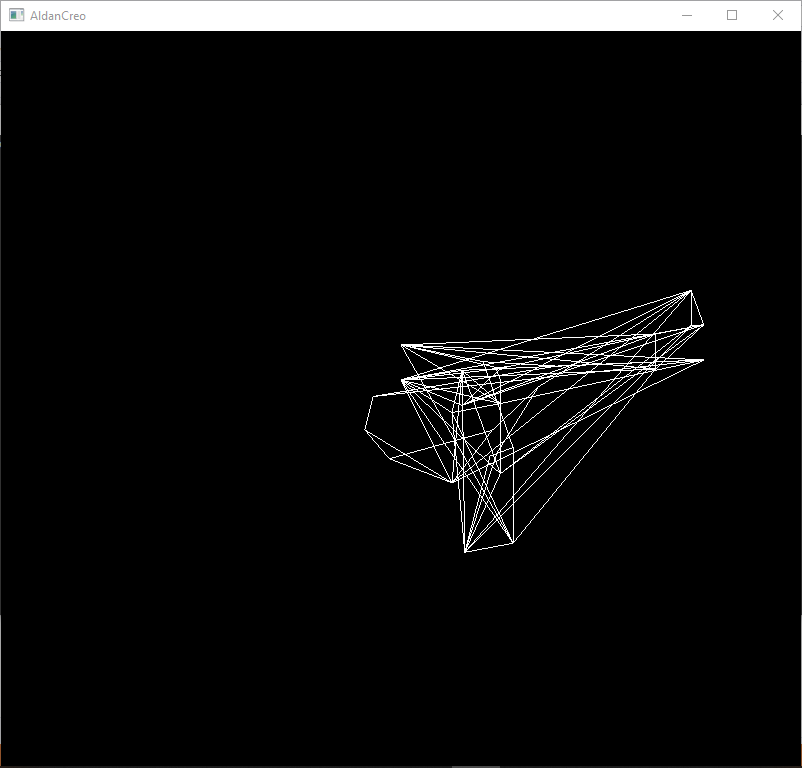
\includegraphics{Penrose_1_no_funciona.png}
    }
    \caption{Visualización de la aplicación en etapas previas del desarrollo, antes de tener en cuenta que el indexado de vértices, normales y texturas, en el formato \texttt{.obj}, empieza en 1.} \label{antes_de_corregir_indexado}
\end{figure}

\subsection{Pespectiva y visión}

La perspectiva que elegido para desarrollar la aplicación es la ortográfica (isométrica), ya que es necesaria para desarrollar este tipo de ilusiones ópticas. He calculado los ángulos adecuados para posicionar la cámara, y los he guardado como un vector que uso a la hora de dibujar para indicar la posición de la cámara.

\subsection{Posicionado} \label{posicion}

\begin{figure}[h]
    \centering
    \resizebox*{0.4\textwidth}{!}{
    
\includegraphics{esfera_posicion_lejos.png}
    }
    \caption{Posición de la esfera: $(470, 430, 230)$.} \label{esfera_posicion_lejos}
\end{figure}
\begin{figure}[h]
    \centering
    \resizebox*{0.4\textwidth}{!}{
    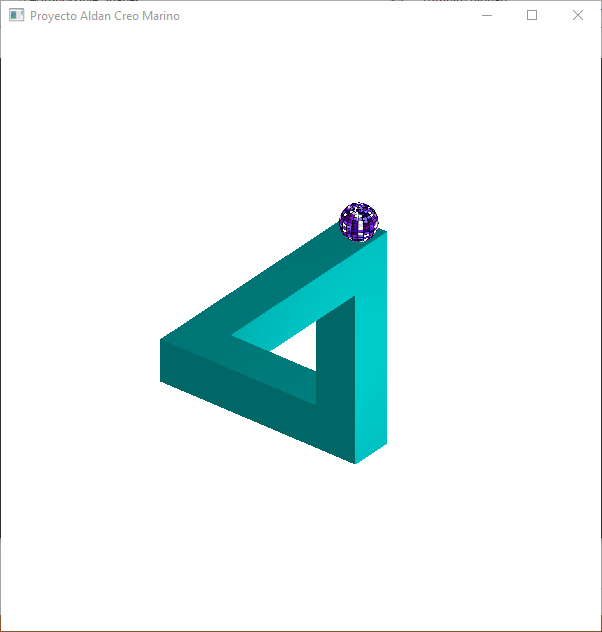
\includegraphics{esfera_posicion_cerca.png}
    }
    \caption{Posición de la esfera: $(35, 70, -270)$.} \label{esfera_posicion_cerca}
\end{figure}

Para posicionar los elementos, he tenido que hacerlo manualmente, ya que precisamente en esta aplicación, al jugar con ilusiones ópticas, las coordenadas 3D aparentes no se corresponden con las reales. Por ejemplo, cuando en el recorrido que hace la esfera automáticamente, esta pasa de la posición \ref{esfera_posicion_lejos} a la posición \ref{esfera_posicion_cerca}, realmente está haciendo un movimiento mucho más grande de lo que parece. Como digo, esto es por el juego óptico que hace la aplicación. Por este motivo, el cálculo de las coordenadas de la esfera lo he hecho de forma manual.

\subsection{Iluminación}

He decidido aplicar iluminación de distintas formas a la esfera y al triángulo. Para eso uso dos shaders separados.

Con respecto a la esfera, como realmente se está moviendo en el espacio 3D de una forma distinta a la que aparenta, no puedo colocar una luz en un lugar de la escena, ya que según la esfera se va moviendo, la luz le daría desde ángulos distintos a los que el usuario espera, dando una impresión extraña en su movimiento, ya que es un movimiento irreal. Frente a esto, probé tres posibles enfoques. El primero fue elegir un ángulo para la luz constante. En este caso, la iluminación no parecía demasiado real, pero el resultado era aceptable. El segundo fue colocar la luz en una posición muy lejana, para que a la esfera no le afecte mucho el cambio de ángulo mientras se mueve en el espacio 3D. Este enfoque produjo resultados aceptables. Pese a todo, mi decisión final fue quedarme sólo con iluminación ambiental (al 100\% de intensidad) para la esfera, ya que como la textura que le apliqué es de una esfera de discoteca, creo que es lógico que la propia esfera no sea iluminada externamente.

Con respecto al triángulo, le he aplicado iluminación ambiental más atenuada que a la esfera, y también iluminación difusa. En este caso, no considero que el efecto que produce la iluminación difusa parezca irreal.

\subsection{Texturizado} \label{texturizado}

Como ya he comentado, he decidido aplicarle una textura de esfera de discoteca a la esfera, y no aplicarle ninguna textura al triángulo (aunque sí sería posible, ya que he realizado el mapeado de las tres mallas). De esta forma, considero que se parece un poco más al juego en que basé mi idea (\ref{hocus}).

En la aplicación, uso dos shaders separados, uno que aplica texturizado y otro que no.

\subsection{Interpolador} \label{interpolador}

Para que la esfera se mueva entre las distintas posiciones automáticamente, he creado una clase que se encarga de realizar automáticamente los cálculos de interpolación entre distintas posiciones.

Esto lo hace usando un algoritmo lineal, al que se le indica un tiempo máximo para realizar la interpolación, una posición de partida, y una posición de destino. La clase se encarga de realizar todos los cálculos necesarios para permitir el movimiento. En toda la aplicación, solo se utiliza una clase encargada de realizar interpolaciones, ya que solo es la esfera que está en movimiento.

\subsection{Controlador de la esfera} \label{controlador_esfera}

También he creado una clase que se encarga de controlar todos los aspectos referidos al movimiento de la esfera, no solo la interpolación entre las posiciones individuales de su trayectoria. Esta clase se ayuda del interpolador (\ref{interpolador}).

Concretamente, lo que incluye es una lista de las posiciones por las que tiene que ir pasando la esfera, y le pide al interpolador que se encargue de realizar la interpolación entre cada una de las posiciones de su trayectoria. Además, cuando alcanza cualquiera de sus destinos, le indica al interpolador que pase a calcular la interpolación para llegar a la siguiente posición.

Adicionalmente, mantiene información sobre el estado actual de movimiento de la esfera, que se guarda como números correspondientes a cada pequeña trayectoria dentro del recorrido general, del 0 al 13.

La información sobre el estado actual se utiliza para saber qué partes del triángulo hay que pintar por encima de la esfera y cuál es no, para conseguir el efecto 3D deseado, usando el algoritmo del pintor. Este proceso lo describo a continuación.

\subsection{Algoritmo del pintor} \label{algoritmo_pintor}

Dado que en la aplicación jugamos con ilusiones ópticas, y las coordenadas 3D aparentes no se corresponden con las reales (\ref{posicion}), he tenido que recurrir a una aplicación manual del algoritmo del pintor para conseguir un efecto realista de la ilusión del triángulo de Penrose. Si usase el pintado en base al buffer de profundidad, la bola aparecería por encima o por debajo de algunas partes del triángulo de forma incorrecta, quitándole el efecto realista a la aplicación. Es decir, hace falta controlar de forma manual el orden de pintado de los objetos, para que la ilusión óptica sea realista.

Para ello, sirviéndonos de la información del estado actual de movimiento de la esfera (\ref{controlador_esfera}), podemos saber qué partes del triángulo se deben pintar en cada momento por encima de la misma, y cuáles no.

\begin{figure}[h]
    \centering
    \resizebox*{0.4\textwidth}{!}{
    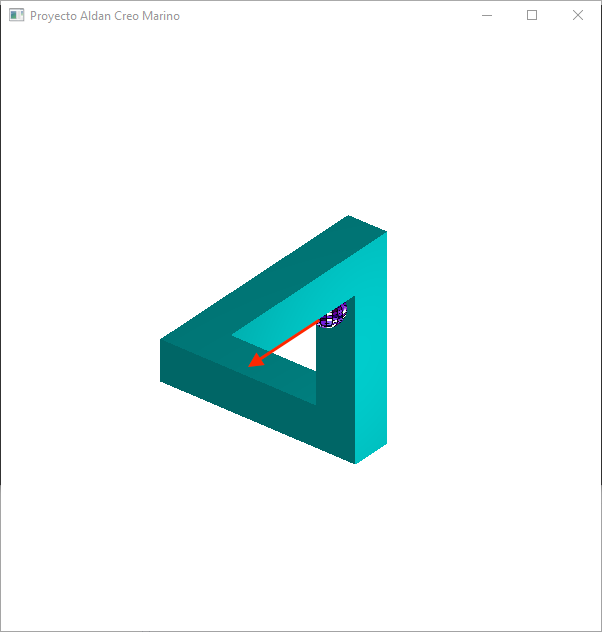
\includegraphics{estado_1.png}
    }
    \caption{Posición de la esfera al principio del movimiento. Se muestra \textbf{por encima} del segmento más oscuro del triángulo.} \label{estado_1}
\end{figure}
\begin{figure}[h]
    \centering
    \resizebox*{0.4\textwidth}{!}{
    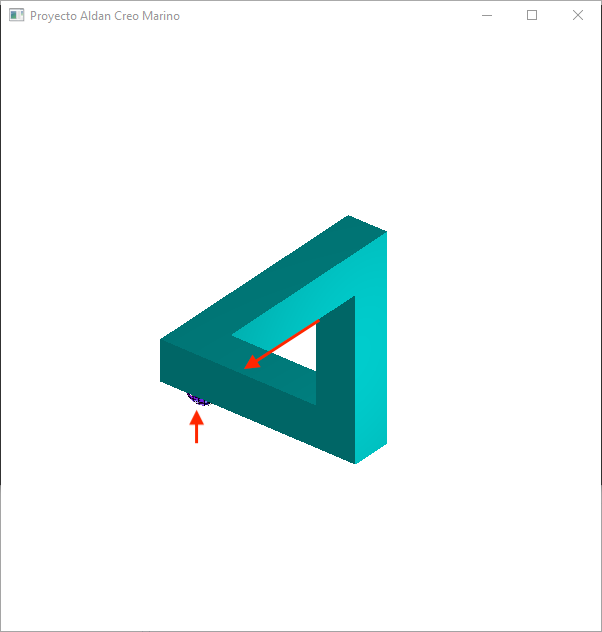
\includegraphics{estado_2.png}
    }
    \caption{Posición de la esfera al final del movimiento. Se muestra \textbf{por debajo} del segmento más oscuro del triángulo.} \label{estado_2}
\end{figure}

Por ejemplo, en las figuras \ref{estado_1} y \ref{estado_2} vemos que, siendo parte del mismo movimiento, en una parte, la cara oscura del triángulo se pinta por debajo de la esfera, y en la otra, se pinta por encima.

La forma de implementar este efecto es dividiendo el movimiento en dos, por lo que en la primera parte la cara oscura se pinta por debajo, y en la segunda parte se hace al revés. Por tanto, hay un cambio en algún punto intermedio de la trayectoria, en el orden de dibujo de los objetos de la aplicación. Concretamente, la transición se hace en un punto intermedio en el que la bola no está tocando con la cara implicada, de forma que la transición no se nota.

Este tipo de estrategia la aplico en varios puntos a lo largo de la trayectoria de la esfera, para conseguir el efecto óptico que busco.

También es relevante comentar, como punto final, que el algoritmo del pintor se puede aplicar en este caso porque no existen caras ocultas en los objetos. Si existieran, al realizar el pintado de forma manual, algunas de las caras se verían superpuestas a las que deberían aparecer realmente por encima. Como describí en \ref{edicion_blender}, eliminé las caras ocultas del modelo, precisamente por esta razón.

\section{Comentarios finales}

En la aplicación, he incluido la posibilidad de mover manualmente la esfera, pero si se usa esa posibilidad, hay que tener en cuenta que el movimiento resulta bastante extraño. Esto es debido a la ilusión óptica con la que juega la aplicación. Los controles se encuentran en el apéndice \ref{controles}.

En la entrega del proyecto he incluido tanto el ejecutable, como los ficheros fuente que se pueden usar para compilar el proyecto.

\newpage
\section{Bibliografía}
\bibliography{export}

\newpage
\appendix
\section{Controles de la aplicación} \label{controles}

Los controles de la aplicación son los siguientes:

\begin{itemize}
    \item \textbf{P}: forzar el algoritmo del pintor para el dibujo, dibujando la esfera por encima.
    \item Posicionado de la esfera:
    \begin{itemize}
        \item \textbf{M}: activar o desactivar el posicionado manual de la esfera.
        \item \textbf{Q}: incrementar manualmente la coordenada X de la esfera.
        \item \textbf{A}: decrementar manualmente la coordenada X de la esfera.
        \item \textbf{W}: incrementar manualmente la coordenada Y de la esfera.
        \item \textbf{S}: decrementar manualmente la coordenada Y de la esfera.
        \item \textbf{E}: incrementar manualmente la coordenada Z de la esfera.
        \item \textbf{D}: decrementar manualmente la coordenada Z de la esfera.
    \end{itemize}
    \item Control de la cámara:
    \begin{itemize}
        \item \textbf{$\uparrow$}: inclinar la cámara hacia arriba manualmente.
        \item \textbf{$\downarrow$}: inclinar la cámara hacia abajo manualmente.
        \item \textbf{$\rightarrow$}: inclinar la cámara hacia la derecha manualmente.
        \item \textbf{$\leftarrow$}: inclinar la cámara hacia la izquierda manualmente.
    \end{itemize}
\end{itemize}

\textit{(No recomiendo jugar con la perspectiva de la cámara, ya que se pierde el efecto de la ilusión óptica, pero he decidido mantener la posibilidad de hacerlo.)}

\end{document}